\documentclass{article}
\usepackage{tikz}
\usetikzlibrary{arrows}
\begin{document}
 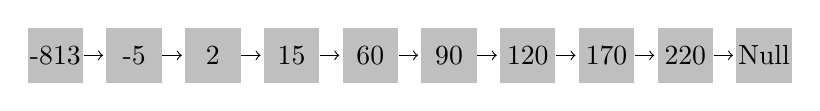
\begin{tikzpicture}[shorten >=1pt,->]
 \tikzstyle{main_node}=[rectangle,fill=black!25,minimum size=20pt,inner sep=0pt] 
\node[main_node] (1) {-813}; 
\node[main_node] (2)[right of=1] {-5}; 
\node[main_node] (3)[right of=2] {2}; 
\node[main_node] (4)[right of=3] {15}; 
\node[main_node] (5)[right of=4] {60}; 
\node[main_node] (6)[right of=5] {90}; 
\node[main_node] (7)[right of=6] {120}; 
\node[main_node] (8)[right of=7] {170}; 
\node[main_node] (9)[right of=8] {220}; 
\node[main_node] (null) [right of=9] {Null};

\path[every node/.style={font=\sffamily\small}]
(1) edge [left] node [left] {} (2)
(2) edge [left] node [left] {} (3)
(3) edge [left] node [left] {} (4)
(4) edge [left] node [left] {} (5)
(5) edge [left] node [left] {} (6)
(6) edge [left] node [left] {} (7)
(7) edge [left] node [left] {} (8)
(8) edge [left] node [left] {} (9)
(9) edge [left] node [left] {} (null);


 \end{tikzpicture} 
\end{document}
